\chapter{LƯU ĐỒ GIẢI THUẬT VÀ CHƯƠNG TRÌNH}

\section{Lưu đồ giải thuật}

    Lưu đồ giải thuật dùng cho chương trình được mô tả trên \fig{\ref{Fig:flowchart}}:

    \begin{figure}[htp]
        \begin{center}
            \hspace*{-1cm}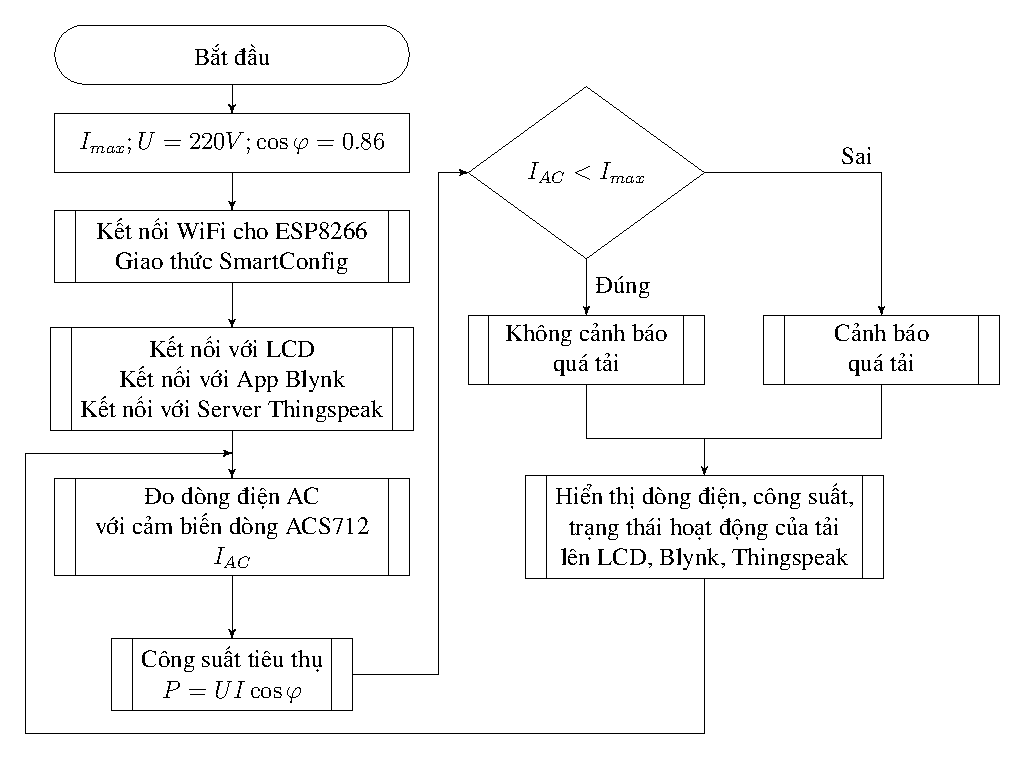
\includegraphics[scale=1]{flowchart.pdf}
            % \subimport{../flowchart/}{flowchart.tex}
        \end{center}
        \caption{Sơ đồ khối thiết kế bộ điều khiển} \label{Fig:flowchart}
    \end{figure}

\section{Chương trình điều khiển}
    \lstinputlisting{acs712_arduino.ino}

\section{Kết quả thu được}
    \begin{figure}[htp]
        \begin{center}
            \hspace*{-1cm}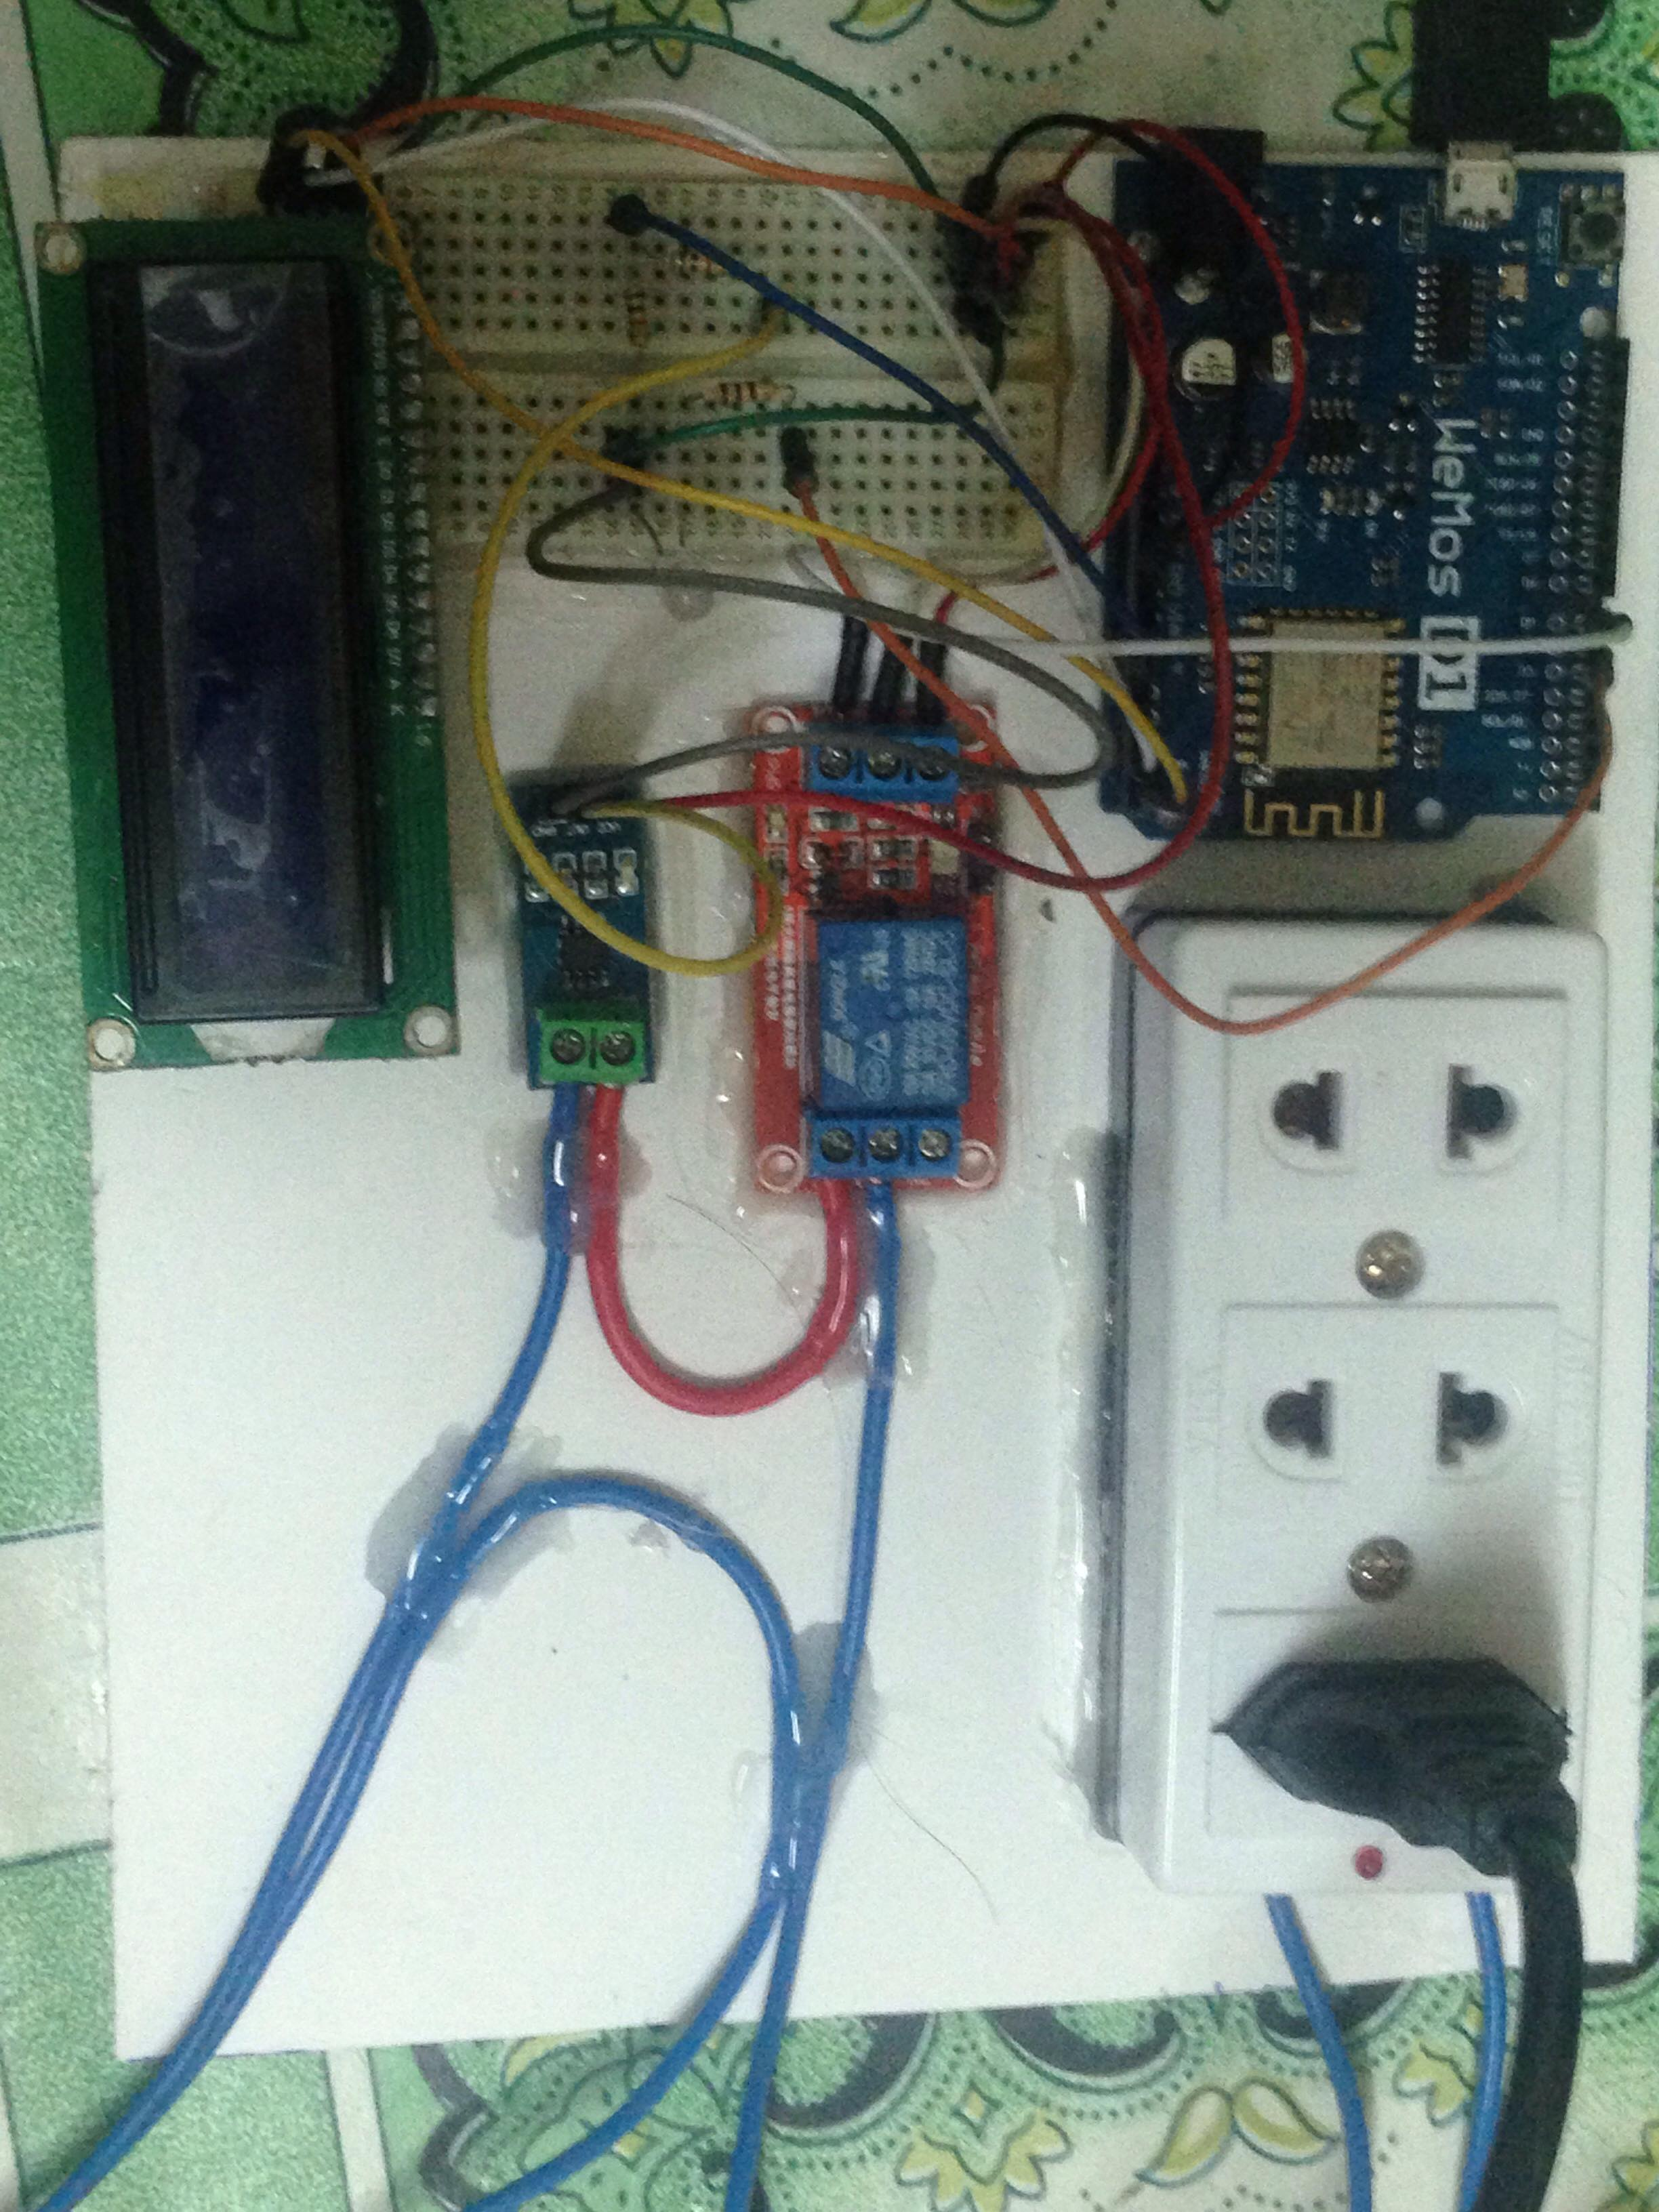
\includegraphics[scale=.08]{hardware-1}
            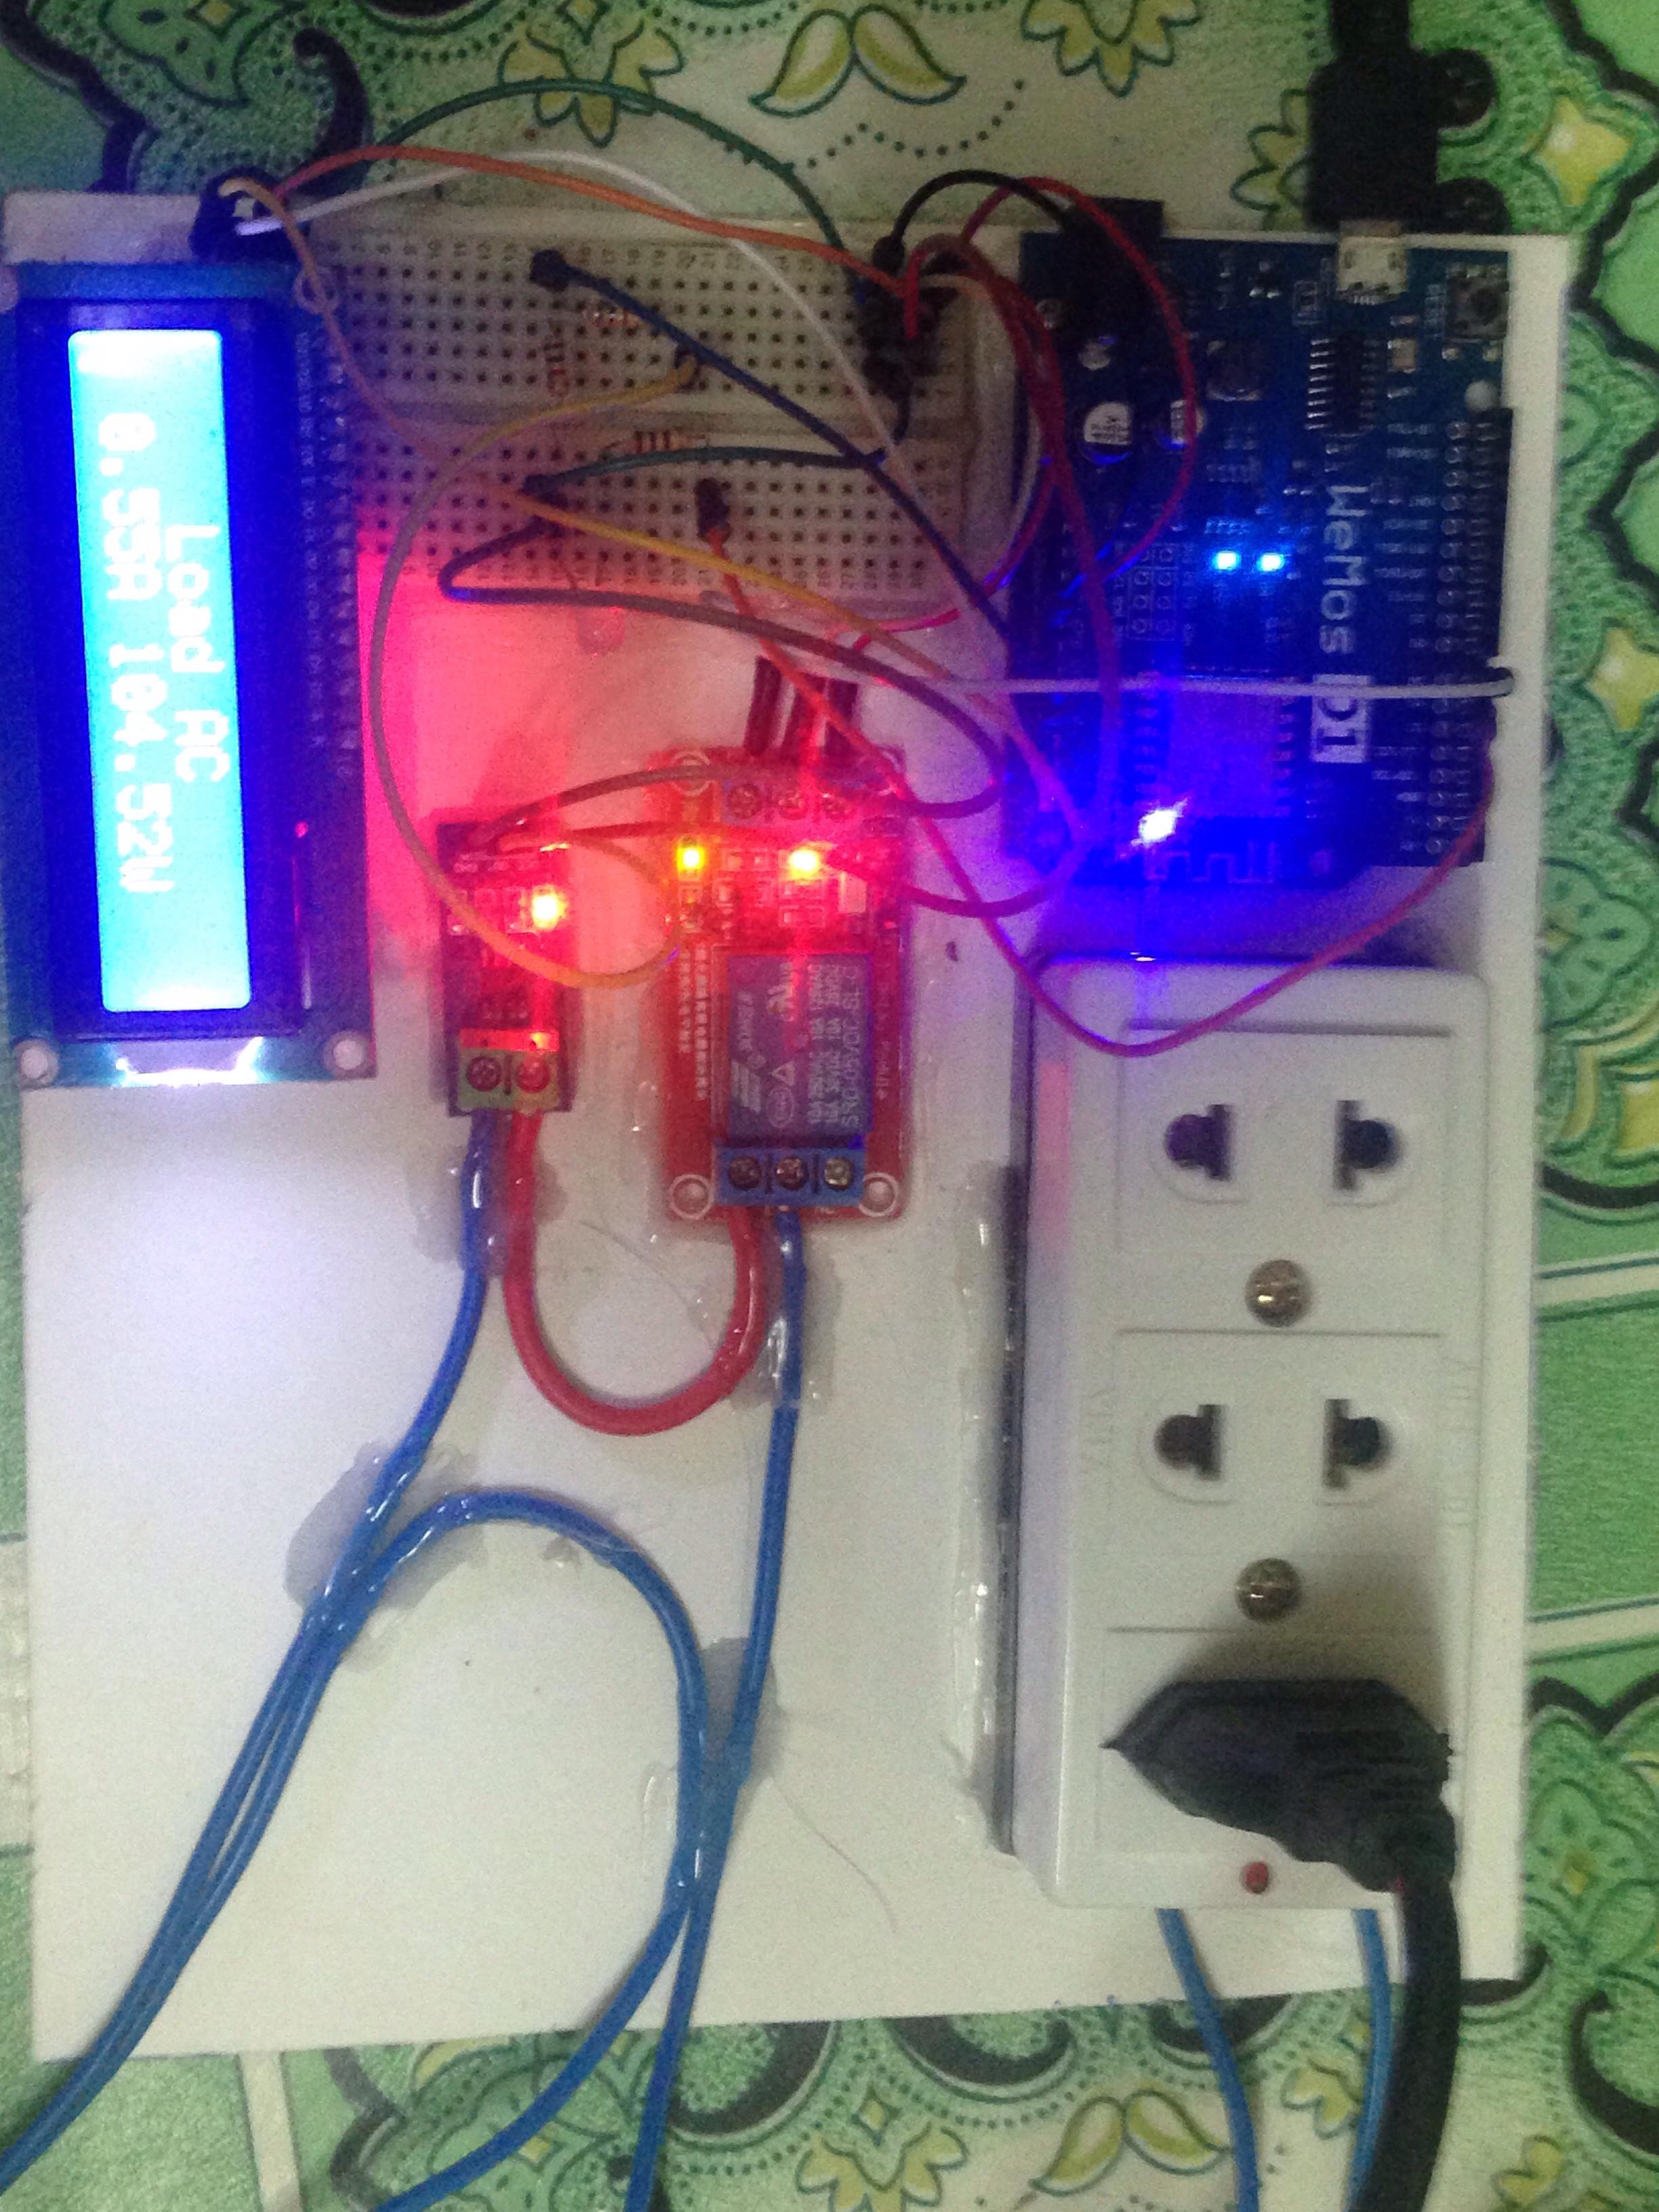
\includegraphics[scale=.08]{hardware-2}
        \end{center}
        \caption{Kết quả thu được về phần cứng} \label{Fig:result}
    \end{figure}

    \begin{figure}[htp]
        \begin{center}
            \subfloat[Kết quả trên Blynk]
                {
                    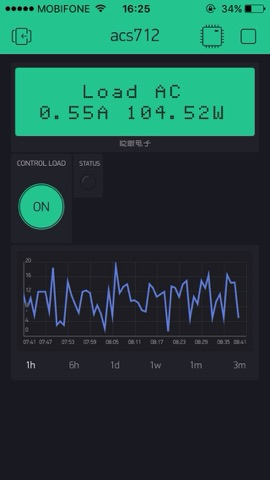
\includegraphics[scale=.5]{blynk-result}
                }
            \subfloat[Kết quả dòng điện trên Thingspeak]
                {
                    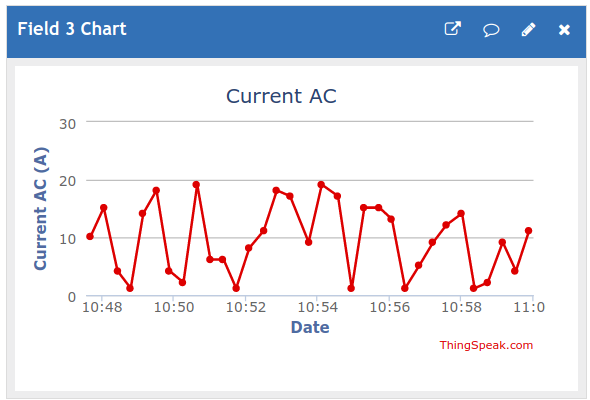
\includegraphics[scale=.5]{Current_Thingspeak}
                }\\

            \subfloat[Kết quả công suất trên Thingspeak]
                {
                    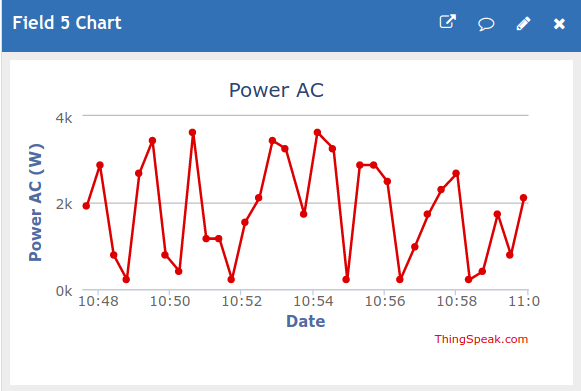
\includegraphics[scale=.35]{Power_Thingspeak}
                }
            \subfloat[Kết quả trạng thái quá tải trên Thingspeak]
                {
                    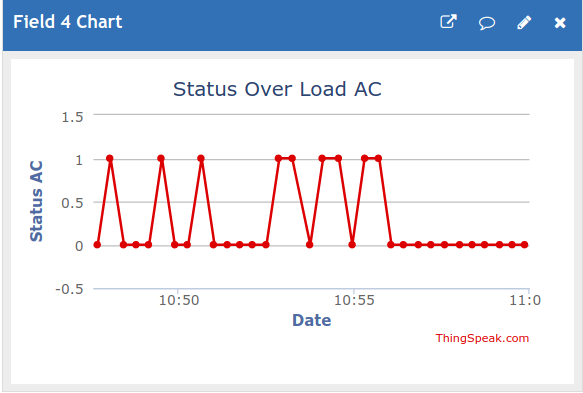
\includegraphics[scale=.35]{Status_Overload_Thingspeak}
                }
        \end{center}
        \caption{Kết quả thu được quan sát trên ứng dụng} \label{Fig:result}
    \end{figure}
